%% LyX 2.1.1 created this file.  For more info, see http://www.lyx.org/.
%% Do not edit unless you really know what you are doing.
\documentclass[12pt,a4paper,oneside,english]{amsbook}
\usepackage[T1]{fontenc}
\usepackage[latin9]{inputenc}
\pagestyle{headings}
\setcounter{secnumdepth}{5}
\setcounter{tocdepth}{5}
\usepackage{babel}
\usepackage{amsthm}
\makeindex
\usepackage{graphicx}
\usepackage{setspace}
\onehalfspacing
\usepackage[unicode=true,pdfusetitle,
 bookmarks=true,bookmarksnumbered=false,bookmarksopen=false,
 breaklinks=false,pdfborder={0 0 1},backref=false,colorlinks=false]
 {hyperref}

\makeatletter

%%%%%%%%%%%%%%%%%%%%%%%%%%%%%% LyX specific LaTeX commands.
\pdfpageheight\paperheight
\pdfpagewidth\paperwidth


%%%%%%%%%%%%%%%%%%%%%%%%%%%%%% Textclass specific LaTeX commands.
\numberwithin{section}{chapter}
\numberwithin{equation}{section}
\numberwithin{figure}{section}
\newenvironment{lyxcode}
{\par\begin{list}{}{
\setlength{\rightmargin}{\leftmargin}
\setlength{\listparindent}{0pt}% needed for AMS classes
\raggedright
\setlength{\itemsep}{0pt}
\setlength{\parsep}{0pt}
\normalfont\ttfamily}%
 \item[]}
{\end{list}}

\makeatother

\begin{document}

\title{SKB and skb-gdbus}


\date{22.07.14}
\begin{abstract}
The first proof-of-concept implementation of the knowledge base leveraged
by Barrelfish project in Linux. Normal session bus is used as a placeholder
for the name, and name ``org.freedesktop.skb'' is used as IPC interface
for the caller. Internally, EcliPSe Prolog implementation and its
C library interface are used as a container of the key-value database,
with internal constraint solving engine. Pre-requisites, current functionality,
and limitations are described in respective chapters of this document.

\newpage{}
\end{abstract}

\maketitle
\tableofcontents{}


\section*{The SKB concept.}


\subsection*{Definition and purpose}

Most of the information from this chaptes is extracted from Barrelfish
related research and respective thesis 


\urladdr{http://e-collection.library.ethz.ch/eserv/eth:6969/eth-6969-02.pdf }

A universal container of system-relevant data is represented as a
new Linux user space daemon which we will call System Knowledge Base
(SKB). It should operate as a central high level system description
database AND constraint solver/script engine for applications and
OS/runtime. It is accessed via IPC by the application and OS/R \textendash{}
both for adding facts/scripts (called queries) to it and then later
running those queries over the facts to get \textquotedblleft knowledge\textquotedblright{}
out of the system. Possible queries are for example finding the best
placement of an application based on NUMA memory access patterns,
scheduling strategies, adaption/scaling of an application on different
platforms, etc.

The concept is based on an implementation from a research multi-kernel
OS called Barrelfish 


\urladdr{www.barrelfish.org}

The purpose of the SKB is providing a general storage for high-level
declarative facts as well as an execution environment to execute declar-
ative algorithms. The goal of the SKB is to serve as a central point
where the OS, drivers and applications collect all information which
might be interesting not only for themselves, but also for other modules.
The SKB provides a uniform and standardized way of querying hardware
informa- tion and software state to OS components and applications.
By using high- level facts, services and applications do not need
to know specific details about how to get access to information registers
of devices. They also do not need to worry about how to interpret
hardware information, which is usually provided as bit fields in registers.
High-level facts provide the in- formation of interest in a register-layout-independent
way. Facts are there- fore easy to read by machines, and even by humans,
and they always have the same format, independently of how the hardware
manufacturer decided to expose the information on the particular piece
of hardware by registers. Another purpose of the SKB is forming a
basis to build reasoning algo- rithms. These algorithms describe a
higher-level problem based on stored facts. Additionally to stored
facts, parameters can be passed to algorithms. Parameters are the
better choice over stored facts, if their values change quickly. On
top of stored facts, rules combine several facts to produce new, high-level
knowledge. This new knowledge can be further processed by higher-level
reasoning algorithms which describe a complete problem


\subsection*{Examples}

The cache is an important part of the hardware which significantly
af- fects software\textquoteright s performance, depending on whether
it is used the right way or not. Cache information is provided by
the SKB as high-level facts, which means that properties such as cache
size, cache line size, level or associativity can be queried independently
of the actual CPU architecture. It is the SKB\textquoteright s responsibility
(together with its datagathering services de- scribed in section 3.5.3)
to get the information using the appropriate low- level mechanism.
On x86 CPUs, the cpuid instruction provides cache in- formation in
an encoded way, while on other architectures there are other low-level
mechanisms to gather low-level data or the information might even
come from online measurements instead of information registers. At
the end it does not matter to the clients, how the cache facts were
pro- duced, as long as the client can query the SKB for cache line
sizes, as- sociativity and other properties important to the application
in a uniform and abstracted way. The current CPU utilization is one
example of information which changes quickly. It is better to pass
this value as argument rather than storing and constantly updating
it as fact in the SKB. NUMA-aware allocation makes use of a simple
reasoning algorithm. Finding the destination core\textquoteright s
NUMA region involves combining the core\textquoteright s a affinity
domain with the memory region. The reasoning algorithm in the SKB
derives an allocation policy which gets passed to the actual memory
allocator. The memory allocator only provides nism of allocating memory.
With the derived allocation policy in the SKB, the memory allocator
can be instructed to allocate memory from a specific range (which
is not necessarily the calling core\textquoteright s local memory).
Not only memory appears in the physical address range, but also many
devices export their registers through a memory mapping to be set
up by the operating system. Algorithms to derive policies on where
to map which device run in the SKB based on facts about available
physical ad- dress space and facts about device properties and their
dependencies. PCIe allocation is one of the most complex problems
of allocating physical ad- dress space. A detailed description of
the PCIe configuration and its policy code to derive physical address
allocation based on available address win- dows and device requirements
is given in section 6. The SKB derives not only lower-level policies,
like memory and phys- ical address range policies, it also derives
policies for complete higher- level problems described in CLP. As
an example, applications describe what properties in terms of hardware
resources they would like to meet. A high-level description of application
requirements and available hardware allows the OS to derive a core
to application mapping. 


\section*{Linux SKB representation}


\subsection*{Architecture and pre-requisits}

As described above, SKB leverages EcliPSe Prolog engine as a back-end,
therefore it should be installed on the target before skb is build.
If it is not install, the compilation will fail due to missing Include
files. The ``standard'' location of the EcliPSe package is 
\begin{lyxcode}
/usr/local/eclipse
\end{lyxcode}
In case installation path is different, it needs to be defined in
CMakeLists.txt as ECLIPSE\_DIR. The Makefiles generated should then
pick up that and provide proper CFLAGS and LDFLAGS, bud YMMV. To see
exact commands cmake is executing, use
\begin{lyxcode}
make~VERBOSE=1
\end{lyxcode}
For d-bus, or, specifically, gdbus - its interlal implementation from
gio-2.x is in use. That means, that gio-2-x-devel (or respective package
un Ubuntu-based Linux that is responsible to install respective headers
and pkg-config macros) needs to be installed. The glib2 library will
be probably installed as a dependency to gio2, but if not - it needs
to be installed explicitly, as some gdbus instantiated code is going
to be generated from xml file, using gdbus-codegen. On Fedora systems,
that is part of glib2-devel, on others, if cmake will complain about
missing gdbus-codegen - the proper package needs to be figured out
and installed.


\subsection*{Getting EcliPSe running}

All relevant information is described on the project website


\urladdr{www.eclipseclp.org}

Basically, installation boils down to run the RUNME script, supplied
with the tarball. It is recommended to put the needed libraries directory
(for required architecture) into ld.so.conf, so that dynamic linker
will be able to locate the library. Path to the eclipse binary itself
is good to have, but not required. Although it should be handled by
the makefile, required CFLAGS and LDFLAGS are
\begin{lyxcode}
-I\$ECLIPSE\_DIR/inlcude/\$ARCH~

-leclipse~-L\$ECLIPSE\_DIR/lib/\$ARCH
\end{lyxcode}

\subsection*{Putting daemon on gdbus}

Similar to CORBA in its early days, gdbus uses declarative xml to
generate bunch of utility code. The format is self explanatory and
looks as follows
\begin{lyxcode}
<?xml~version=\textquotedbl{}1.0\textquotedbl{}~encoding=\textquotedbl{}UTF-8\textquotedbl{}~?>~

<node~name=\textquotedbl{}/\textquotedbl{}~xmlns:doc=\textquotedbl{}http://www.freedesktop.org/dbus/1.0/doc.dtd\textquotedbl{}>~~~

~~<interface~name=\textquotedbl{}org.freedesktop.skb\textquotedbl{}>

~~~~<method~name=\textquotedbl{}AddFact\textquotedbl{}>

~~~~~~<arg~name=\textquotedbl{}fact\textquotedbl{}~type=\textquotedbl{}s\textquotedbl{}~direction=\textquotedbl{}in\textquotedbl{}~~/>

~~~~~~<arg~name=\textquotedbl{}reply\textquotedbl{}~type=\textquotedbl{}s\textquotedbl{}~direction=\textquotedbl{}out\textquotedbl{}~~/>

~~~~</method>

~~~~<method~name=\textquotedbl{}Query\textquotedbl{}>

~~~~~~<arg~name=\textquotedbl{}query\textquotedbl{}~type=\textquotedbl{}s\textquotedbl{}~direction=\textquotedbl{}in\textquotedbl{}~~/>

~~~~~~<arg~name=\textquotedbl{}reply\textquotedbl{}~type=\textquotedbl{}s\textquotedbl{}~direction=\textquotedbl{}out\textquotedbl{}~~/>

~~~~</method>

~~~~<property~name=\textquotedbl{}Activated\textquotedbl{}~type=\textquotedbl{}b\textquotedbl{}~access=\textquotedbl{}read\textquotedbl{}~/>

~~</interface>~

</node>
\end{lyxcode}
Here we have 2 methods - AddFact and Query, both taking and returning
string values. For the first one, returned value mostly represents
if a fact has been successfully inserted into database or there was
a error, for secod one - it is logical result of CLP execution, and
either error output or normal output if there were no error condition
triggered. 

If all the pre-requisites for compilation were met, simple make should
build the skb binary. If something does not quite work, exact flags
could be looked up in compile.sh script residing in contrib/ directory. 

The code which is necessary to get a handle on the d-bus is generated
from the xml file above. In our case, cmake will present 
\begin{lyxcode}
Generating~Skb.h,~Skb.c
\end{lyxcode}
with respective files should appear in the project directory. The
callback functions (or gdbus methods implementation) resides in file
\begin{lyxcode}
skb\_gdbus.c
\end{lyxcode}
The code first tries to own a name on the d-bus. If the name is busy,
or that is not possible by other means, the on\_name\_aquired() callback
function never gets called, and on\_name\_lost() gets called with
NULL as the connection parameter. In that case, we stop the main loop,
since the requested name is not available. In order to work directly
with EcliPSe part of the code without d-bus interaction, sample implementation
could be found in contrib/ directory. 

There is no output from the skb application unless something gone
wrong, or debug options are toggled (this is controlled by GLOBAL\_DEBUG
define - similar to Barrelfish. 


\subsection*{Testing the SKB}

As there is no direct interface to skb, d-bus is required to get skb
to work. dbus-send and other d-bus controlling utilities could be
used, as well as custom application with d-bus interface. For testing
purpose, major Linux distributions provide ``d-feet'' application.

Testing sequence is as follows.
\begin{itemize}
\item Start the skb application (if it is not built, run make first)
\item If the app does not exit with error, it should be ready to service
d-bus requests
\item Start the d-feet application. It should look similar to the below
\begin{figure}
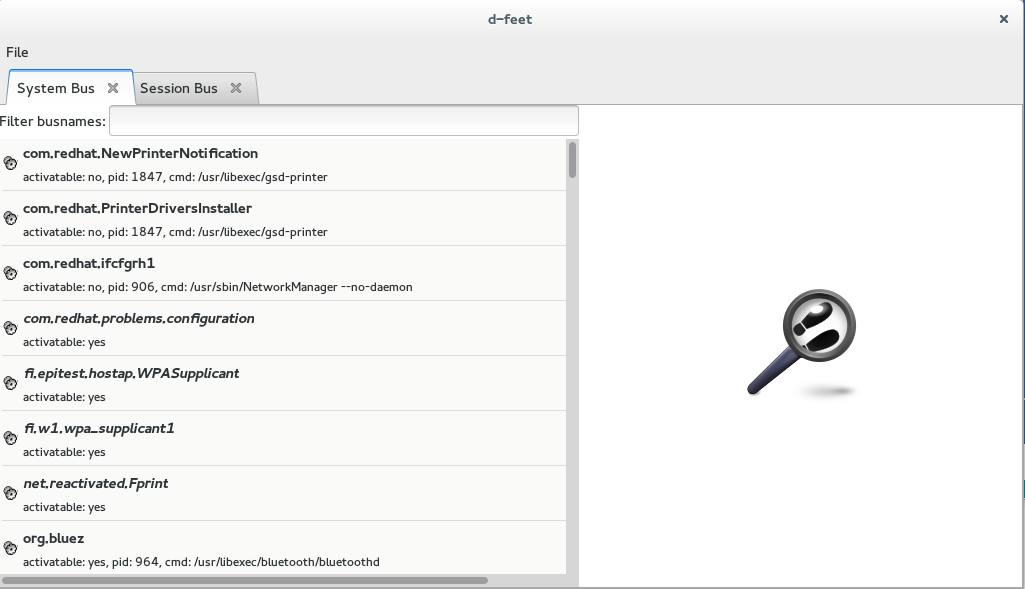
\includegraphics[width=0.7\paperwidth]{Pictures/Screenshot_1}

\protect\caption{d-feet application}
\end{figure}

\item Switch to Session Bus, and locate the Skb there
\item Select Skb, then on right hand side serviced d-bus methods will appear
\end{itemize}
\begin{figure}
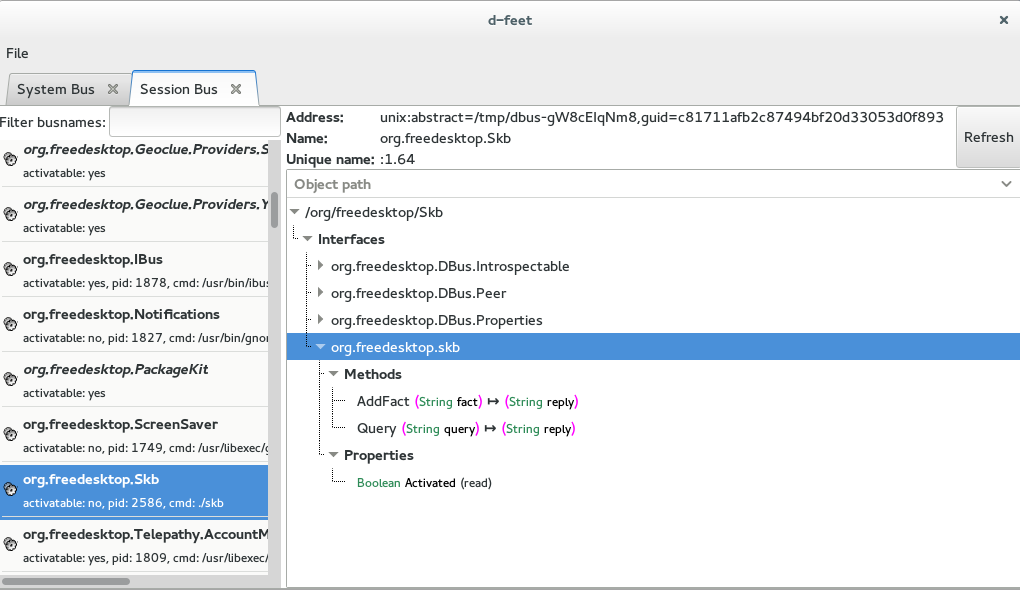
\includegraphics[width=0.6\paperwidth]{Pictures/Screenshot_2}

\protect\caption{Skb methods instrospection}
\end{figure}

\begin{itemize}
\item double-click on the method will open a dialog, which enables to execute
selected method, and see its return output. 
\end{itemize}

\printindex{}
\end{document}
